% This example is meant to be compiled with lualatex or xelatex
% The theme itself also supports pdflatex
\PassOptionsToPackage{unicode}{hyperref}
\documentclass[aspectratio=1610, 12pt]{beamer}

% Warning, if another latex run is needed
% \usepackage[aux]{rerunfilecheck}

% just list chapters and sections in the toc, not subsections or smaller
\setcounter{tocdepth}{1}

%------------------------------------------------------------------------------
%------------------------------ Fonts, Unicode, Language ----------------------
%------------------------------------------------------------------------------
\usepackage{fontspec}
\defaultfontfeatures{Ligatures=TeX}  % -- becomes en-dash etc.

% german language
\usepackage{polyglossia}
\setdefaultlanguage{german}

% for english abstract and english titles in the toc
\setotherlanguages{english}

% intelligent quotation marks, language and nesting sensitive
\usepackage[autostyle]{csquotes}

% microtypographical features, makes the text look nicer on the small scale
\usepackage{microtype}

%------------------------------------------------------------------------------
%------------------------ Math Packages and settings --------------------------
%------------------------------------------------------------------------------

\usepackage{amsmath}
\usepackage{amssymb}
\usepackage{mathtools}
\usepackage{bbold}

% Enable Unicode-Math and follow the ISO-Standards for typesetting math
\usepackage[
  math-style=ISO,
  bold-style=ISO,
  sans-style=italic,
  nabla=upright,
  partial=upright,
]{unicode-math}
\setmathfont{Latin Modern Math}

% nice, small fracs for the text with \sfrac{}{}
\usepackage{xfrac}


%------------------------------------------------------------------------------
%---------------------------- Numbers and Units -------------------------------
%------------------------------------------------------------------------------

\usepackage[
  locale=DE,
  separate-uncertainty=true,
  per-mode=symbol-or-fraction,
]{siunitx}
\sisetup{math-micro=\text{µ},text-micro=µ}
% \sisetup{tophrase={{ to }}}
%------------------------------------------------------------------------------
%-------------------------------- tables  -------------------------------------
%------------------------------------------------------------------------------

\usepackage{booktabs}       % \toprule, \midrule, \bottomrule, etc

%------------------------------------------------------------------------------
%-------------------------------- graphics -------------------------------------
%------------------------------------------------------------------------------

\usepackage{graphicx}
%\usepackage{rotating}
\usepackage{grffile}
\usepackage{tikz}
\usepackage{circuitikz}
\usepackage{tikz-feynman}
\usepackage{subcaption}

% allow figures to be placed in the running text by default:
\usepackage{scrhack}
\usepackage{float}
\floatplacement{figure}{htbp}
\floatplacement{table}{htbp}

% keep figures and tables in the section
\usepackage[section, below]{placeins}

% smileys
\usepackage{MnSymbol,wasysym}

%------------------------------------------------------------------------------
%---------------------- customize list environments ---------------------------
%------------------------------------------------------------------------------

\usepackage{enumitem}
\usepackage{listings}
\usepackage{hepunits}

\usepackage{pdfpages}
%------------------------------------------------------------------------------
%------------------------------ Bibliographie ---------------------------------
%------------------------------------------------------------------------------

\usepackage[
  backend=biber,   % use modern biber backend
  autolang=hyphen, % load hyphenation rules for if language of bibentry is not
                   % german, has to be loaded with \setotherlanguages
                   % in the references.bib use langid={en} for english sources
]{biblatex}
\addbibresource{references.bib}  % the bib file to use
\DefineBibliographyStrings{german}{andothers = {{et\,al\adddot}}}  % replace u.a. with et al.


% Load packages you need here
% \usepackage{polyglossia}
% \setmainlanguage{german}

\usepackage{csquotes}


% \usepackage{amsmath}
% \usepackage{amssymb}
% \usepackage{mathtools}

\usepackage{hyperref}
\usepackage{bookmark}

% load the theme after all packages

\usetheme[
  showtotalframes, % show total number of frames in the footline
]{tudo}

% Put settings here, like
\unimathsetup{
  math-style=ISO,
  bold-style=ISO,
  nabla=upright,
  partial=upright,
  mathrm=sym,
}

% \setbeamertemplate{itemize item}{\scriptsize$\blacktriangleright$}
% \setbeamertemplate{itemize subitem}{\scriptsize$\blacktriangleright$}

%Titel:
\title{RTA Update}
%Autor
\author[N.Breer]{Nils Breer}
%Lehrstuhl/Fakultät
\institute{Fakultät Physik}
%Titelgrafik muss ich einfueren!!!
%\titlegraphic{\includegraphics[width=0.3\textwidth]{content/Bilder/interferenz.jpg}}
\date{15.02.2023}

\begin{document}
\maketitle

% 2D node x vs Y plots
\begin{frame}\frametitle{status}
  \begin{itemize}
    \item $\bullet$\, $v1$, $v2$, $\text{low}\mu$ alignments on different runs
    \item $\bullet$\, Alignment quality with residuals per layer
    \item $\bullet$\, nodeX vs nodeY comparison  C-side: most problematic in T2X2 C-side 
  \end{itemize}
\end{frame}

\begin{frame}\frametitle{Mean Residuals}
  \begin{columns}
    \begin{column}[c]{0.33\textwidth}
      \begin{figure}
        \centering
        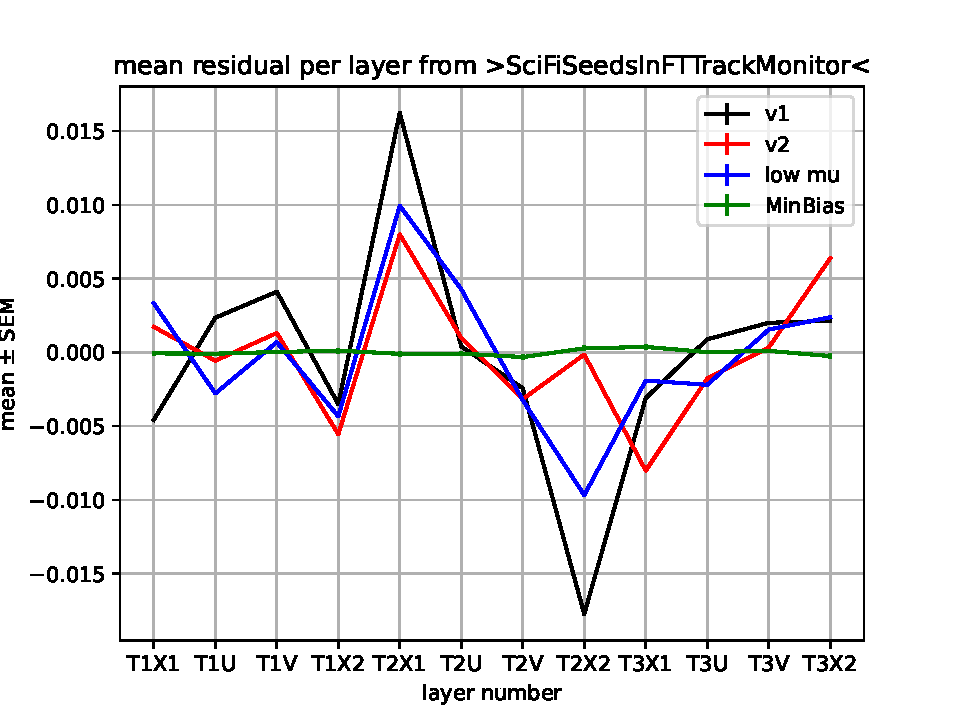
\includegraphics[width=0.9\textwidth]{2023-feb-15/meanResidual_SciFiSeeds_MC_data.pdf}
        \caption{mean Residual per Layer, SciFi Seed Tracks}
      \end{figure}
    \end{column}
    \begin{column}[c]{0.33\textwidth}
      \begin{figure}
        \centering
        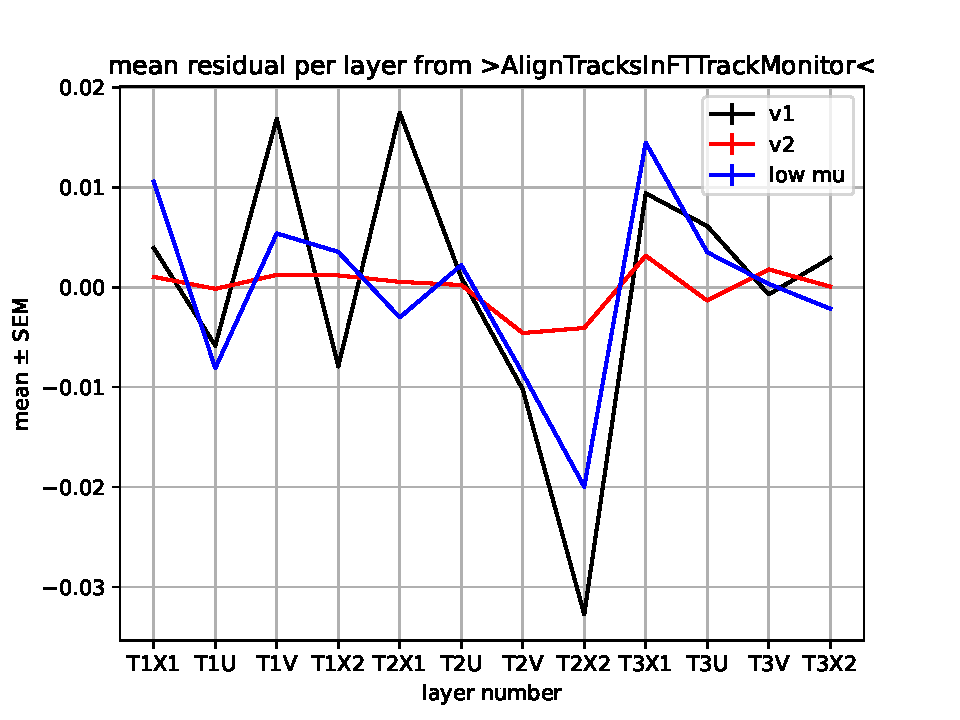
\includegraphics[width=0.9\textwidth]{2023-feb-15/meanResidual_AlignTracks_MC_data.pdf}
        \caption{mean Residual per Layer, weighted Alignment Tracks}
      \end{figure}
    \end{column}
    \begin{column}{0.33\textwidth}
      \begin{itemize}
        \item $\bullet$\, residual on Alignment Tracks is weighted with nHits per quarter to total hits ratio to account for some quarters having fewer hits than others
        \item $\bullet$\, shape of SciFiSeeds and Alignment Tracks comparable (weights. vs no weights, otherwise pretty much the same)
        \item $\bullet$\, second station is problematic
      \end{itemize}
    \end{column}
  \end{columns}
\end{frame}

% \begin{frame}\frametitle{Backup slides}
%   \begin{columns}
%     \begin{column}[c]{0.48\textwidth}
%       \begin{figure}
%         \centering
%         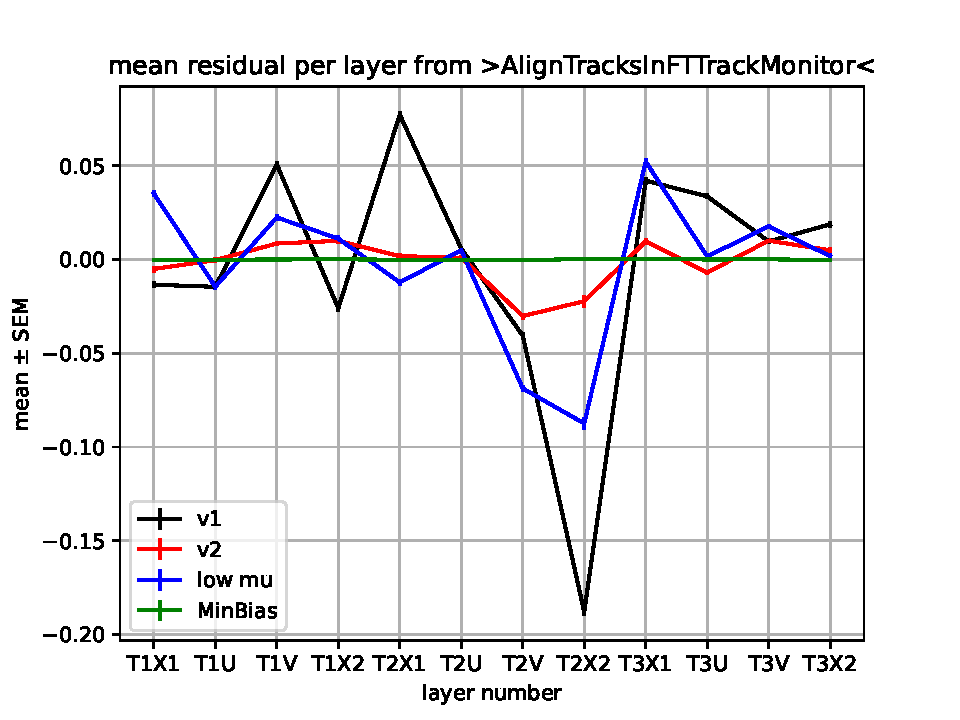
\includegraphics[width=\textwidth]{2023-feb-07/mean_residual_AlignTracks_dataMC.pdf}
%         \caption{mean residuals per layer mean summed quarters.}
%       \end{figure}
%     \end{column}
%     \begin{column}[c]{0.48\textwidth}
%       \begin{figure}
%         \centering
%         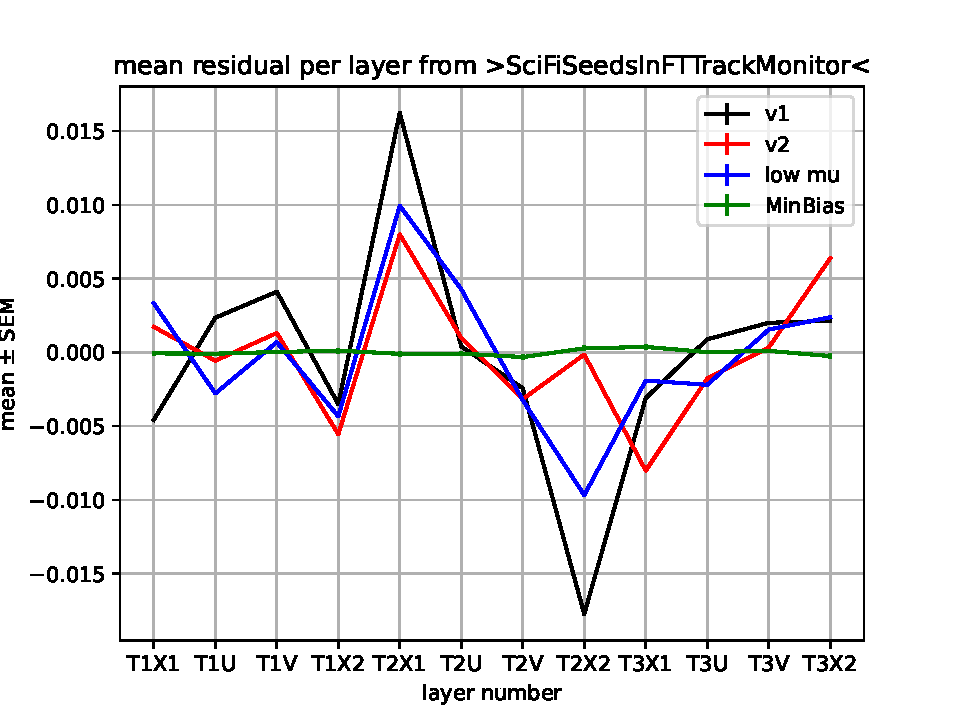
\includegraphics[width=\textwidth]{2023-feb-07/mean_residual_SciFiSeeds_DataVsMC.pdf}
%         \caption{mean residuals per layer mean summed quarters.}
%       \end{figure}
%     \end{column}
%   \end{columns}
% \end{frame}
%
\begin{frame}\frametitle{Residuals for A-side Quarters per Layer}
  \begin{columns}
    \begin{column}[c]{0.48\textwidth}
      \begin{figure}
        \centering
        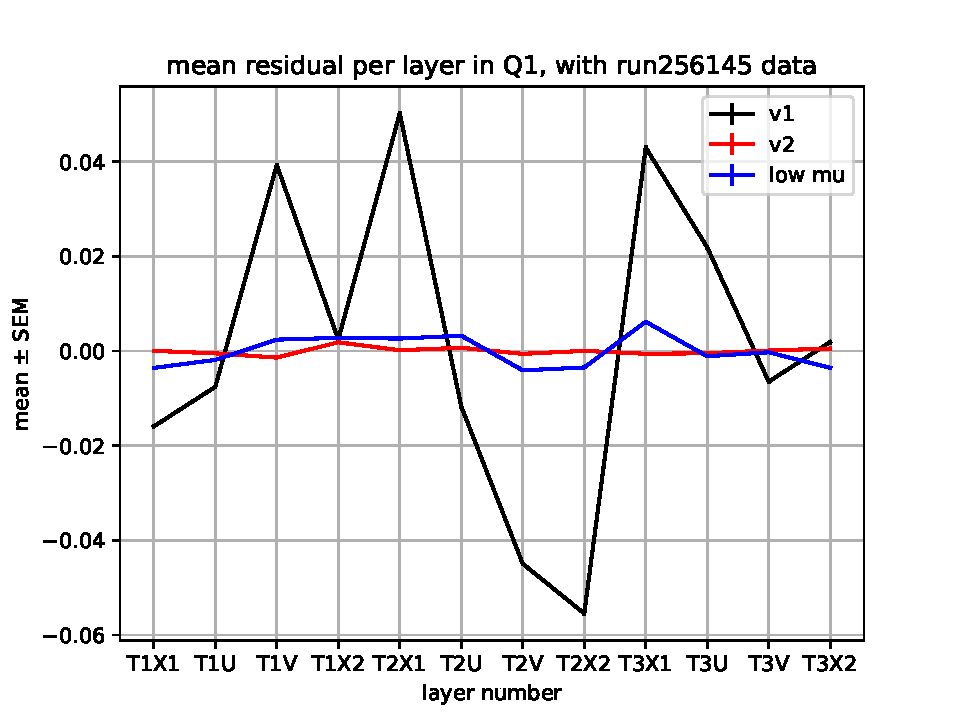
\includegraphics[width=\textwidth]{2023-feb-07/mean_residuals_Q1_allLayers.pdf}
        \caption{mean residuals per layer for Q1.}
      \end{figure}
    \end{column}
    \begin{column}[c]{0.48\textwidth}
      \begin{figure}
        \centering
        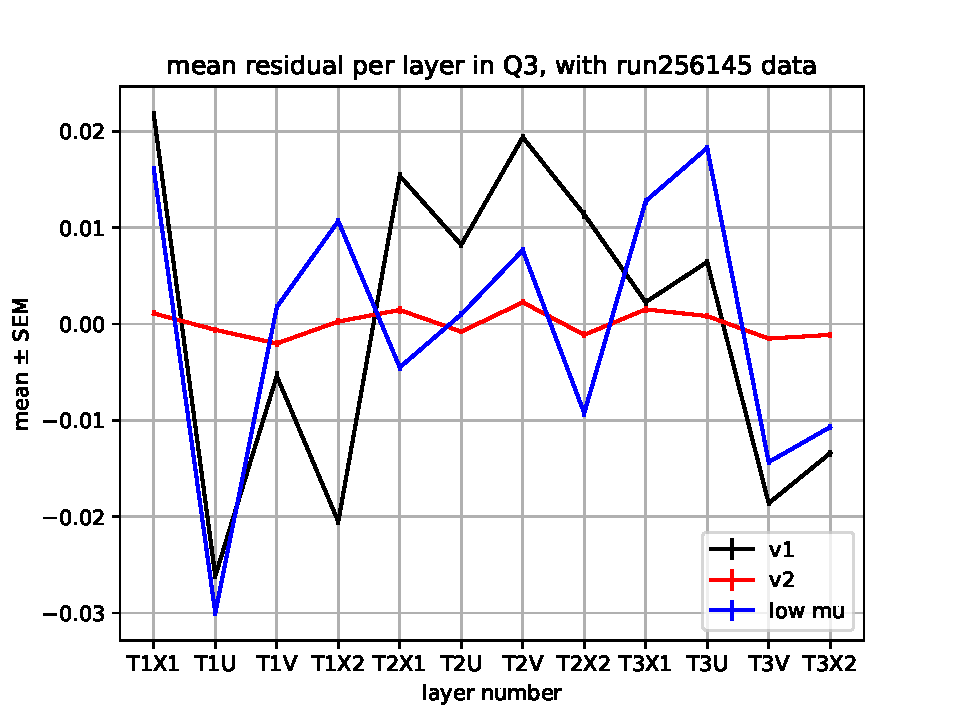
\includegraphics[width=\textwidth]{2023-feb-07/mean_residuals_Q3_allLayers.pdf}
        \caption{mean residuals per layer for Q3.}
      \end{figure}
    \end{column}
  \end{columns}
\end{frame}
%
\begin{frame}\frametitle{Residuals for C-side Quarters per Layer}
  \begin{columns}
    \begin{column}[c]{0.48\textwidth}
      \begin{figure}
        \centering
        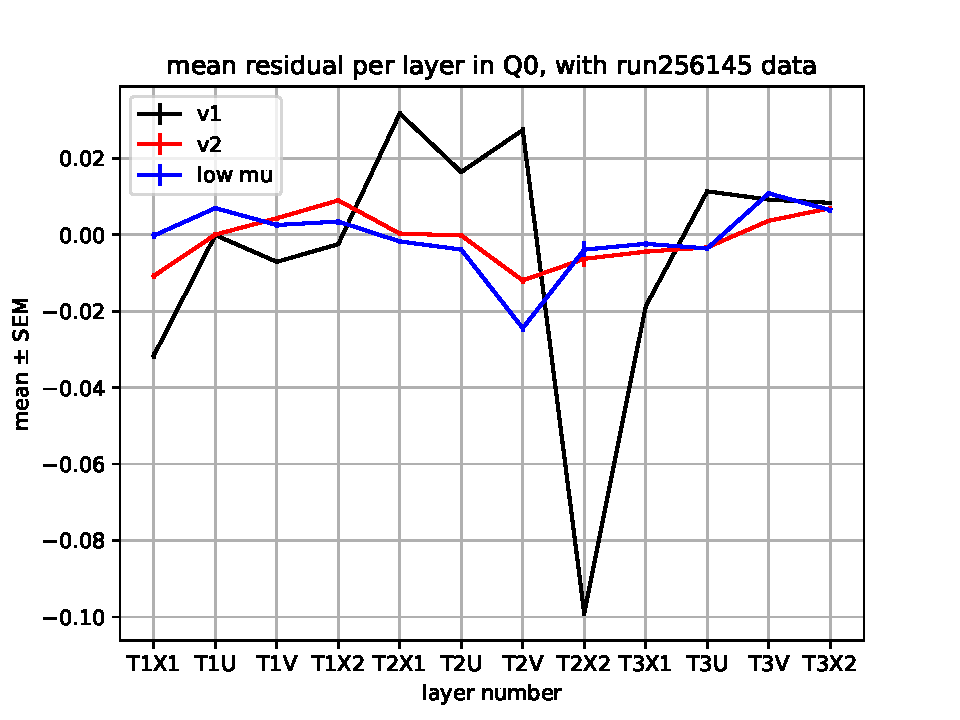
\includegraphics[width=\textwidth]{2023-feb-07/mean_residuals_Q0_allLayers.pdf}
        \caption{mean residuals per layer for Q0.}
      \end{figure}
    \end{column}
    \begin{column}[c]{0.48\textwidth}
      \begin{figure}
        \centering
        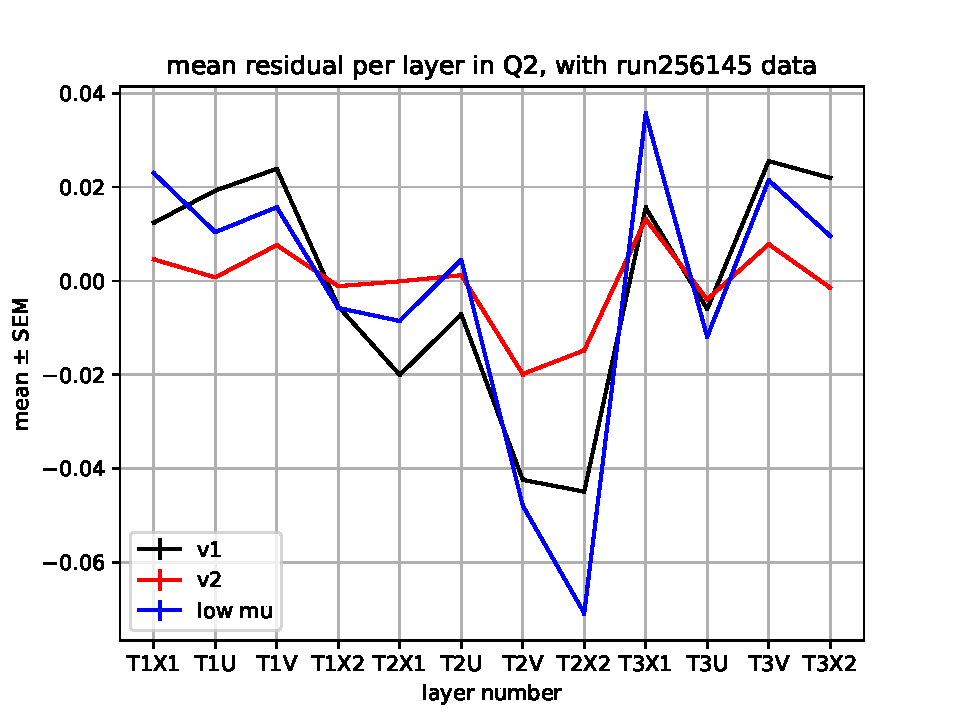
\includegraphics[width=\textwidth]{2023-feb-07/mean_residuals_Q2_allLayers.pdf}
        \caption{mean residuals per layer for Q2.}
      \end{figure}
    \end{column}
  \end{columns}
\end{frame}

\end{document}
